\section{Introduction}

\section{Dévelopemment méthodologique à Chamonix}%
\label{sec:dévelopemment_méthodologique_à_chamonix}

\section{Apportionment method for the oxidative potential of \PMdix{}}

Article paru dans le journal \textit{Atmospheric Chemistry and Physics} le 4 juin 2019 :

\begin{quote}
    Samuël Weber, Gaëlle Uzu, Aude Calas, Florie Chevrier, Jean-Luc Besombes,
    Aurélie Charron, Dalia Salameh, Irena Ježek, Griša Močnik, et Jean-Luc Jaffrezo. 2018.
    \textit{An Apportionment Method for the Oxidative Potential of Atmospheric Particulate
    Matter Sources: Application to a One-Year Study in Chamonix, France}. Atmospheric
    Chemistry and Physics 18(13), pp. 9617‑9629.
    \textsc{doi} : \href{10.5194/acp-18-9617-2018}{https://doi.org/10.5194/acp-18-9617-2018},
    \textsc{url} : \url{https://www.atmos-chem-phys.net/18/9617/2018/}
\end{quote}

\label{sec:weber_et_al_2018}
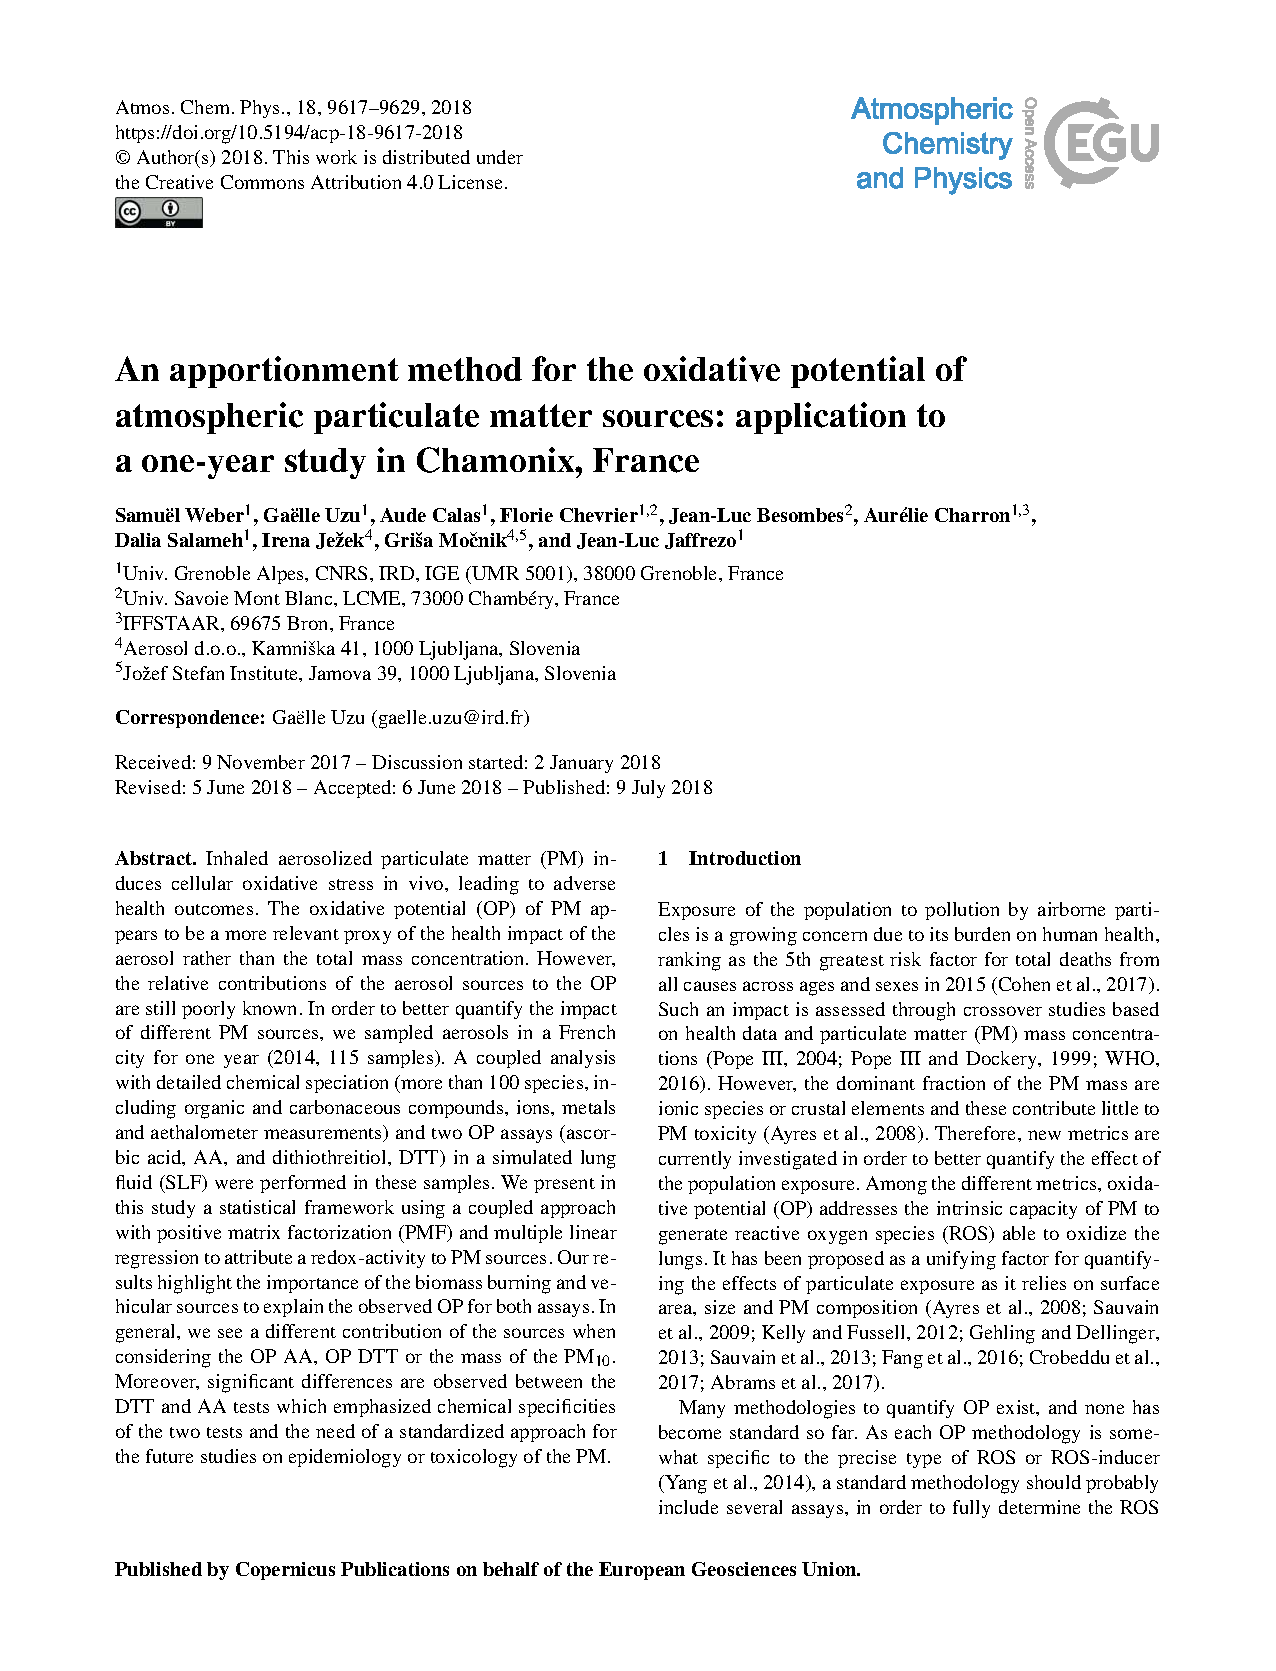
\includepdf[pages=-,scale=0.95,pagecommand={\pagestyle{fancy}}]{chapters/deconvol_OP.pdf}


\section{Conclusion}
